\documentclass[]{beamer}
%\documentclass[handout]{beamer}
%\documentclass[handout,draft]{beamer}
%\documentclass[]{article}


% Preambulo
% Paquetes para usar bien el idioma español
\usepackage[spanish,es-tabla]{babel}
\selectlanguage{spanish}
\usepackage[utf8]{inputenc}

% Paquetes para usar mejores imagenes
\usepackage{graphicx}

% Paquetes para links y tabla de contenidos en el PDF
\usepackage{hyperref}
\hypersetup{colorlinks=true,allcolors=blue}
%\usepackage{hypcap}

% Paquetes para mejores tablas
\usepackage{booktabs}

% Mejor matematica
\usepackage{amsmath}

% Fuentes de las imagenes
\usepackage[absolute,overlay]{textpos}

% Paquete captions
\usepackage[justification=centering,labelformat=empty,labelsep=none]{caption}

% Opciones para ticks
\usepackage{tikz}
\usetikzlibrary{shapes,arrows,positioning}

\tikzstyle{decision} = [diamond, draw, fill=blue!20, text width=4em, text badly centered, node distance=2cm, inner sep=0pt,on grid]
\tikzstyle{block} = [rectangle, draw, fill=blue!20, text width=8em, text centered, rounded corners, minimum height=2em,on grid]
\tikzstyle{line} = [draw, -latex]

% Citas bibliograficas
\usepackage[backend=biber]{biblatex}
\renewcommand{\footnotesize}{\tiny}
\addbibresource{biblio.bib}

% Mejoro las captions
\setbeamertemplate{caption}{\raggedright\insertcaption\par}

\setbeamertemplate{caption}{%
\begin{beamercolorbox}[wd=0.85\paperwidth, sep=.2ex]{block body}\insertcaption%
\end{beamercolorbox}%
}


% Sacar barra de navegacion
\setbeamertemplate{navigation symbols}{}%remove navigation symbols

% Transparencias en items
\setbeamercovered{transparent}

% Estilo de diapositivas
% \usetheme{Boadilla}
\usecolortheme{whale}
\usecolortheme{orchid}

%\usepackage{beamerarticle}

% Titulo
\title{Herramientas de Teledetección Cuantitativa\\{\small Geometría espectral}}
\author{Francisco Nemiña}

\institute{Unidad de Educación y Formación Masiva \\
Comisión Nacional de Actividades Espaciales}

\logo{
\includegraphics[height=0.7cm]{imagenes/sopi.png}}

\AtBeginSection[]
{
\begin{frame}
\frametitle{Esquema de presentación}
\tableofcontents[currentsection]
\end{frame}
}


\begin{document}
\begin{frame}
    \maketitle
\end{frame}

\section{Escenas del capítulo anterior}
\begin{frame}{La vez pasada vimos}
  \begin{itemize}[<+->]
    \item Que a partir de esto podiamos definir la $\rho_\lambda$ la firma espectral como una característica de cada cuerpo.
    \item Definimos 3 tipos de firmas espectrales \emph{patrón} y como se comportaba cada una.
    \item Que es importante corregir a las imágenes atmosfericamente para obtener el valor de reflectancia del píxel.
    \item Que podemos definir índices a partir de hacer operaciones entre los valores de los píxeles como si fueran números.
    \item Que los índices pueden relacionarse con variables en el terreno.
    \item Que podemos entender los índices como mediciones en el espacio espectral.
  \end{itemize}
\end{frame}
%--- Next Frame ---%

\section{Espacio espectral}
\subsection{Operaciones}
\begin{frame}{Pixeles}
  Cada píxel va a tener asociado distintos valores de brillo, uno por banda de adquisición. \pause
  \begin{block}{Definición}
    Hablamos de un vector píxel al vector construido como
    \begin{equation}
      p = (\rho_1, \ldots ,\rho_N)
    \end{equation}
  \end{block}
\end{frame}
%--- Next Frame ---%

\begin{frame}{Operaciones}
  \begin{block}{Operaciones como vectores}
    Podemos:
    \begin{itemize}[<+->]
      \item Sumar
      \item Multiplicar por un número.
      \item \emph{Multiplicar}
    \end{itemize}
  \end{block}
\end{frame}
%--- Next Frame ---%

\begin{frame}{Vectores}
  \begin{block}{Definición}
    Para sumar vectores y multiplicar por un número
    \begin{equation}
      p + \lambda q = (\rho_1+ \lambda \nu_1, \ldots ,\rho_N+\lambda \nu_N)
    \end{equation}
  \end{block}
\end{frame}
%--- Next Frame ---%

\begin{frame}{Base de un espacio}
  \begin{block}{Definición}
    Podemos escribir a un vector
    \begin{equation}
      p = \rho_1 (1,\ldots,0) + \ldots + \rho_N (0,\ldots,1) = \rho_1 e_1 + \ldots + \rho_N e_N
    \end{equation}
    donde los vectores $B = \{e_i, i \in 0, \ldots, N \}$ son la base del espacio espectral
  \end{block}
\end{frame}
%--- Next Frame ---%
\begin{frame}{Base de un espacio}
  \begin{block}{Observación}
    Cambiando la base cambia la representación escrita del vector pero no el vector.
  \end{block}:
  \begin{exampleblock}{Ejemplo}
    Tomemos
    \begin{equation}
      p = (0.4, 0,03)
    \end{equation} en la base $B = \{ (1,0), (0,1)\}$. \pause
    Si ahora tomamos la base $B = \{ (1,1), (1,-1)\}$ lo reescribiremos como
    \begin{equation}
      p = (0.215, 0.185)
    \end{equation}
  \end{exampleblock}
\end{frame}
%--- Next Frame ---%

\subsection{Rotaciones}
\begin{frame}{Rotaciones}
  \begin{block}{Observación}
    Las rotaciones y cambios de escala los podemos pensar como operaciones entre vectores.
  \end{block}:
\end{frame}
%--- Next Frame ---%

\begin{frame}{Matrices}
  \begin{block}{Definición:}
    Las matrices se pueden pensar como transformaciones que convierten a un vector en otro. \pause
    \begin{equation}
      w = Av
    \end{equation}
  \end{block}\pause
  \begin{alertblock}{Propiedad}
    Como las transformaciones que utilizaremos son lineales, con sólo definirlas en unos pocos valores alcanza. \pause Elegir bien los vectores para definir la transformación es útil.
  \end{alertblock}
\end{frame}
%--- Next Frame ---%

\begin{frame}{Ejemplo}
  Empecemos con un ejemplo para una imagen de dos bandas
  \begin{figure}
  \centering
  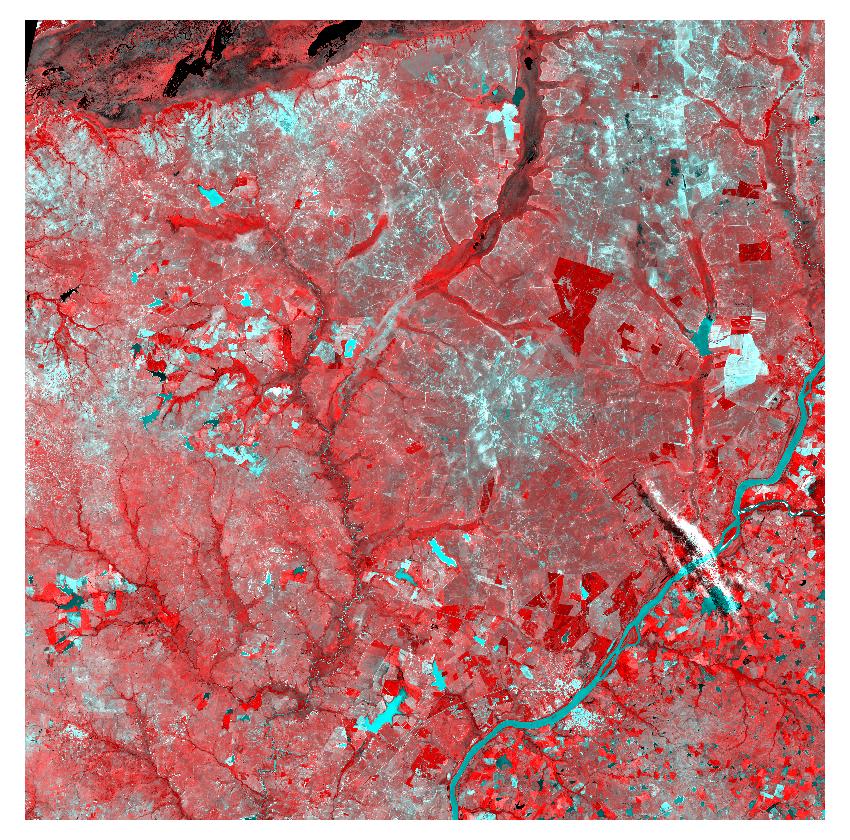
\includegraphics[width=0.6\textwidth]{imagenes/nir-red.png}
  \caption{Imagen de dos bandas.}
  \end{figure}
\end{frame}
%--- Next Frame ---%

\begin{frame}{Idea}
  \begin{figure}
  \centering
  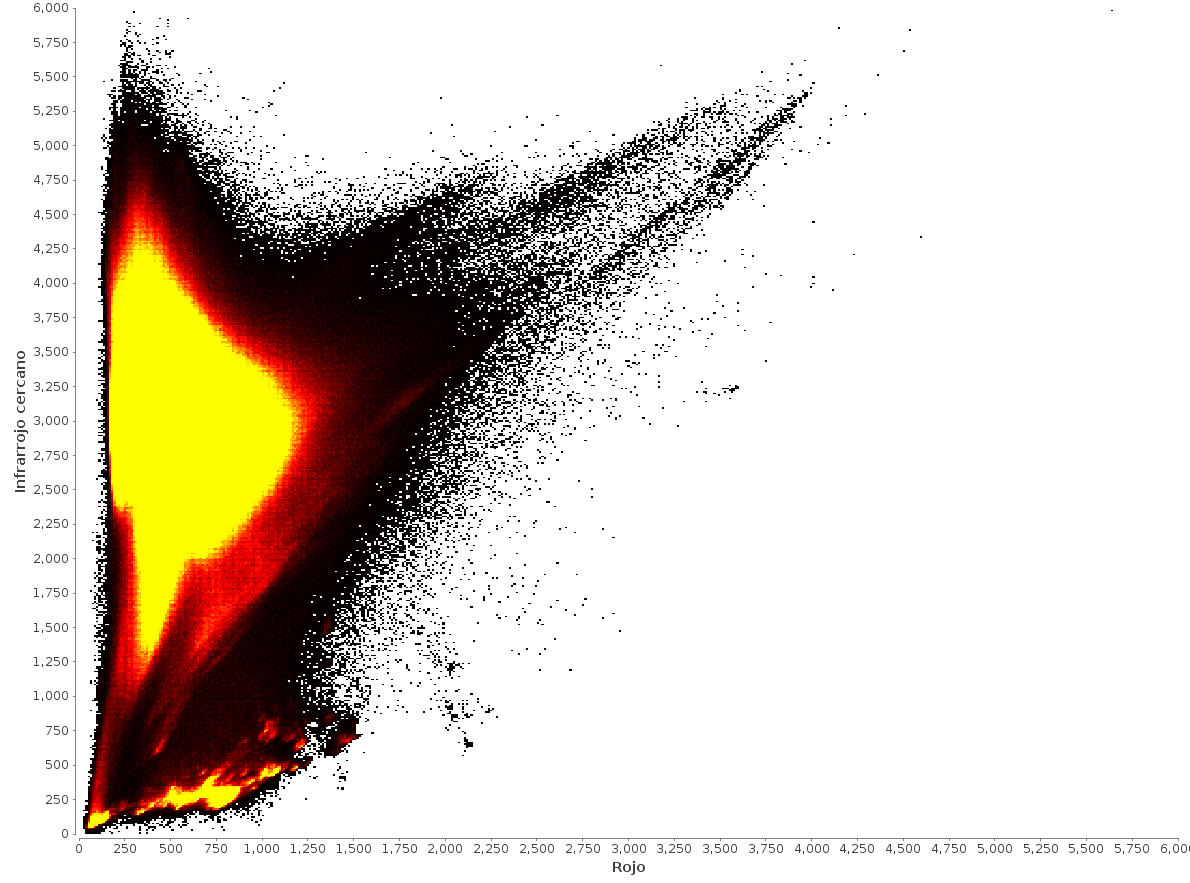
\includegraphics[width=0.8\textwidth]{imagenes/nir-red2.png}
  \caption{Imagen de dos bandas en el espacio vectorial.}
  \end{figure}
\end{frame}
%--- Next Frame ---%

\begin{frame}{Idea}
  \begin{alertblock}{Transformación}
    Una combinación obvia es $$ \rho_d = 0.5\rho_n-0.5\rho_r$$
    y
    $$ \rho_s = 0.5\rho_n+0.5\rho_r $$
  \end{alertblock}
\end{frame}
%--- Next Frame ---%


\section{Componentes principales}
\begin{frame}{Componentes principales}
  \begin{block}{Idea}
    Queremos ver si un set bandas está correlacionadas o no.
  \end{block}
\end{frame}
%--- Next Frame ---%

\begin{frame}{Componentes principales}
  \begin{figure}
  \centering
  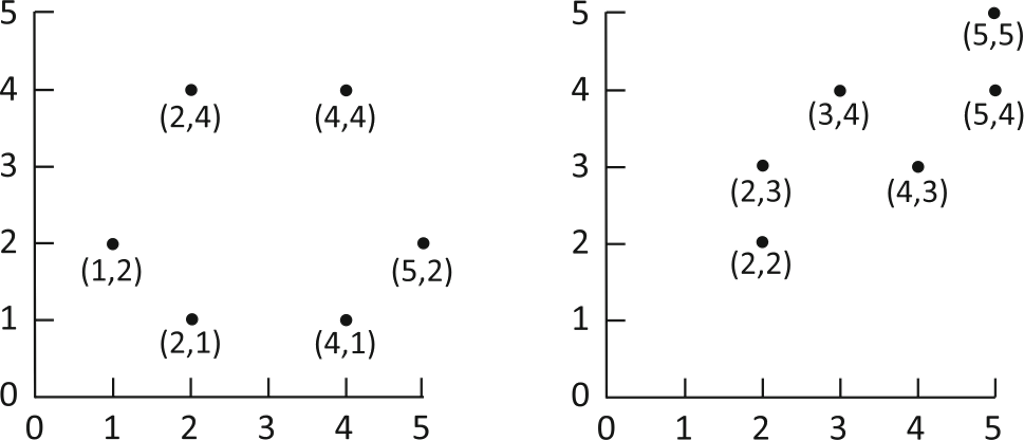
\includegraphics[width=0.8\textwidth]{imagenes/corr.png}
  \caption{Datos correlacionados y no correlacionados\footfullcite{richards2013remote}}
  \end{figure}
\end{frame}
%--- Next Frame ---%

\begin{frame}{Componentes principales}
  \begin{block}{Matriz de correlación}
    Tiene en sus componentes las funciones de correlación entre cada banda\pause
    \[
    A = \begin{bmatrix}
        corr_{11}       & corr_{12} & corr_{13} & \cdots & corr_{1n} \\
        corr_{21}       & corr_{22} & corr_{23} & \cdots & corr_{2n} \\
        \vdots          & \vdots    & \vdots    & \ddots & \vdots \\
        corr_{n1}       & corr_{d2} & corr_{n3} & \cdots & corr_{nn}
    \end{bmatrix} \]
  \end{block}
\end{frame}
%--- Next Frame ---%

\begin{frame}{Componentes principales}
  \begin{block}{Observaciones}
      Queremos que la correlación cruzada entre bandas sea cero.
      \pause\@ Matemáticamente lo pedimos como
        $$Av=\lambda v$$
      Y nos quedamos como vectores útiles a los que cumplan esto.
  \end{block}
\end{frame}
%--- Next Frame ---%

\begin{frame}{Componentes principales}
  \begin{block}{Matriz de correlación}
    La forma de la matriz va a depender de las combinaciones lineal que haga
      entre los vectores \pause\@
    \[\begin{bmatrix}
        \lambda{1}       & 0 & 0 & \cdots & 0 \\
        0       & \lambda_{2} & 0 & \cdots & 0 \\
        \vdots & \vdots & \vdots & \ddots & \vdots \\
        0       & 0 & 0 & \cdots & \lambda_{n}
    \end{bmatrix} \]
    \pause\@
    donde son los autovectores $$\lambda_{1}  > \lambda_{2} > \cdots > \lambda_{n}$$
  \end{block}
\end{frame}
%--- Next Frame ---%

\begin{frame}{Componentes principales}
  \begin{block}{Observaciones}
    \begin{itemize}[<+>]
      \item $\frac{\lambda_i}{\sum_i \lambda_i}$ me habla de cuanto me explica ese vector sobre la variabilidad de la imagen
      \item $(v_1 , \dots , v_n)$ el autovector que me representa la combinación de bandas de un autovalor dado.
      \item Estas combinación lineal de bandas tienen la información más relevante.
    \end{itemize}
  \end{block}
\end{frame}
%--- Next Frame ---%

\begin{frame}{Componentes principales}
  \begin{exampleblock}{Ejemplo}
    Volviendo al ejemplo de antes
    \[
    \begin{bmatrix}
        1       & 0.329127 \\
        0.329127 & 1
    \end{bmatrix} \]
  \end{exampleblock}
\end{frame}
%--- Next Frame ---%

\begin{frame}{Componentes principales}
  \begin{exampleblock}{Ejemplo}
    Al diagonalizar me queda
    \[
    \begin{bmatrix}
        1.343685       & 0 \\
        0       & 0.656315
    \end{bmatrix} \]
    con autovectores $$0.707107\, \rho_n-0.707107 \, \rho_r$$  y $$0.707107 \,
      \rho_n+0.707107\, \rho_r$$ \pause\@
    Acá el primer vector explica el el 67\% de la variabilidad de la imagen y el segundo del 33\%.
  \end{exampleblock}
\end{frame}
%--- Next Frame ---%

\begin{frame}{Componentes principales}
  \begin{figure}
  \centering
  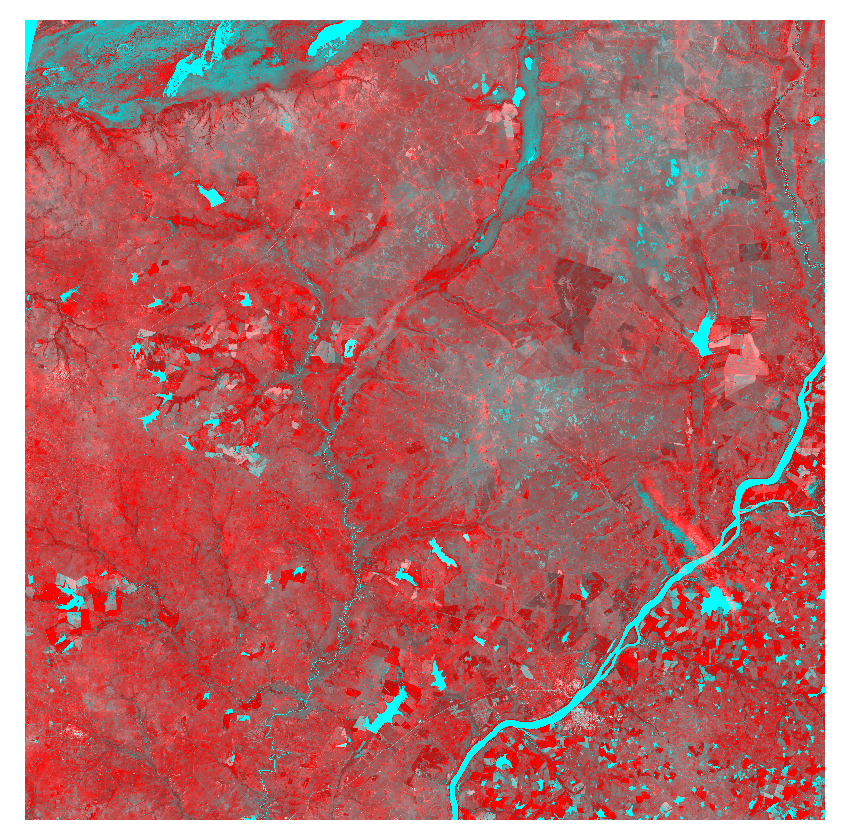
\includegraphics[width=0.6\textwidth]{imagenes/pca1.png}
  \caption{Ejemplo con las bandas nir-rojo en la imagen.}
  \end{figure}
\end{frame}
%--- Next Frame ---%

\begin{frame}{Componentes principales}
  \begin{figure}
  \centering
  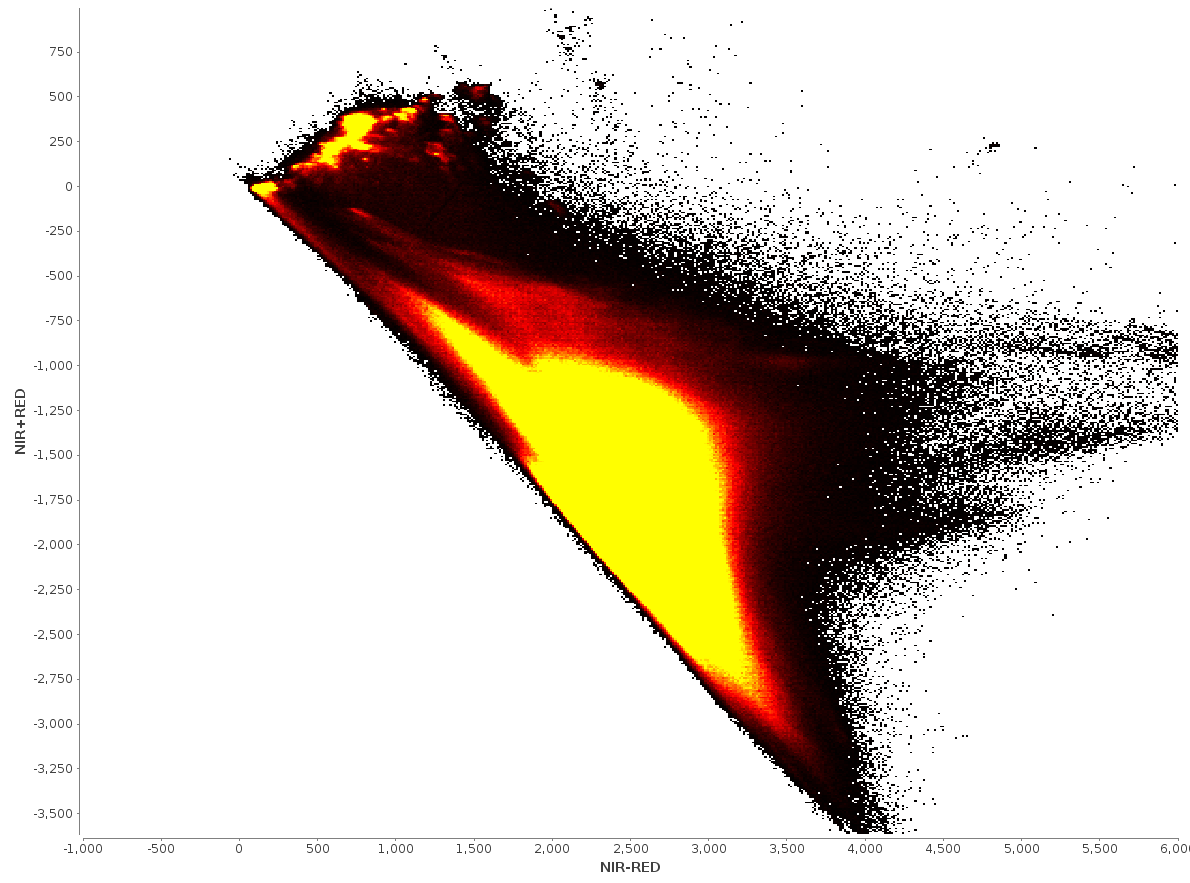
\includegraphics[width=0.8\textwidth]{imagenes/pca2.png}
  \caption{Ejemplo con las bandas nir-rojo en el espacio vectorial.}
  \end{figure}
\end{frame}
%--- Next Frame ---%

\section{Transformada tasseled-cap}

\begin{frame}{Transformada tasseled-cap}
  \begin{block}{Utilidad}
    La utilidad de esto no suele ser con dos bandas, si no con muchas más.
  \end{block}\pause
  \begin{block}{Problema}
    Acá es mas fácil darse cuenta que brinda mas información, el tema es interpretar esa información.
  \end{block}\pause
  \begin{block}{Idea}
    Encontrar alguna transformación que me permita descartar bandas pero que tengan relación con distintos comportamientos biofísicos.
  \end{block}
\end{frame}
%--- Next Frame ---%

\begin{frame}{Transformada tasseled-cap}
  \begin{figure}
  \centering
  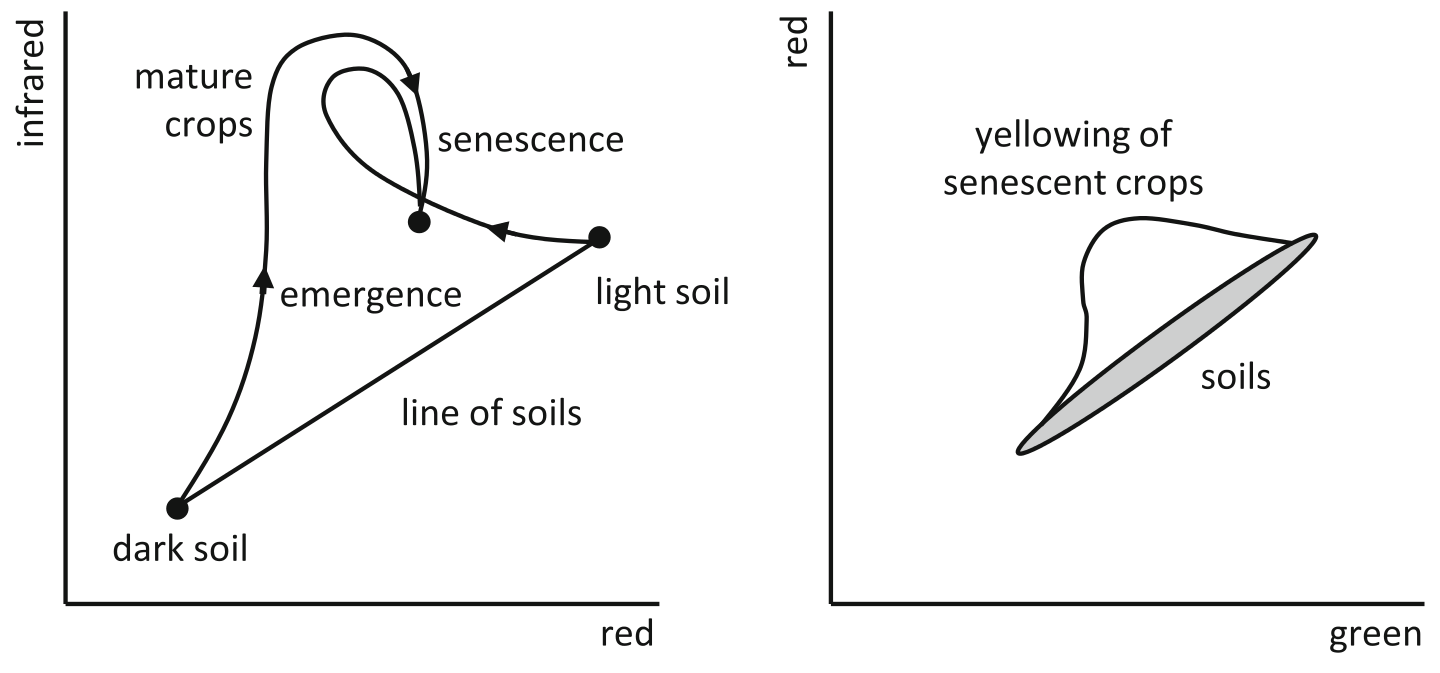
\includegraphics[width=0.8\textwidth]{imagenes/tc.png}
  \caption{Movimiento asociado al comportamiento fenológico de un píxel de vegetación en el espacio vectorial.\footfullcite{richards2013remote}}
  \end{figure}
\end{frame}
%--- Next Frame ---%


\begin{frame}{Transformada tasseled-cap}
    \begin{figure}
      \begin{tabular}{l c c c c c c }
        Combinación  & Azul & Verde & Rojo & nir & swir 1 & swir 2\\
        Brillo &  0.30  & 0.27  & 0.47  & 0.55  & 0.50  & 0.18\\
        Verdor & -0.29  &-0.24  &-0.54  & 0.72 & 0.07  &-0.16\\
        Humedad&  0.15  & 0.19  & 0.32  & 0.34  &-0.71  &-0.45
      \end{tabular}
      \caption{Transformada tasseled-cap para landsat 8 \footfullcite{baig2014derivation}}
    \end{figure}
\end{frame}
%--- Next Frame ---%

\begin{frame}{Transformada tasseled-cap}
  \begin{block}{Idea}
    Todo esto logra hacer que el número de bandas que utilizo sea menor que el
      número de bandas inicial
  \end{block}
\end{frame}
%--- Next Frame ---%

\section{Práctica}

\begin{frame}{Práctica}
  \begin{exampleblock}{Actividades prácticas de la cuarta clase}
    \begin{enumerate}
      \item Calcular la transformada por componentes principales y tasseled-cap sobre la imagen Landsat 8.
      \item Calcular la transformada por componentes principales sobre un apilado de imágenes Landsat 8.
      \item Graficar la variación del EVI a lo largo del año.
      \item Calcular la transforamda por componentes principales al apilado de imágenes EVI.
    \end{enumerate}
  \end{exampleblock}
\end{frame}
%--- Next Frame ---%

\end{document}
